Donnons-nous quatre points $A_1$ , $A_2$ , $A_3$ et $A_4$ sur un cercle, pas forcément distincts, puis pour $n \in \NN_{\geq 5}$ définissons le point $A_n$ comme suit \emph{(d'une certaine façon on essaye de construire un polygone \emph{\og presque régulier \fg})}.
\begin{enumerate}
	\item Si $A_{n-3} \neq A_{n-4}$ alors $\geoset{D} \eqdef (A_{n-3} A_{n-4})$ , sinon $\geoset{D}$ est la tangente en $A_{n-3}$ au cercle.

	\item Soit ensuite $\geoset{D}\,'$ la parallèle à $\geoset{D}$ passant par $A_{n-1}$ . Si $\geoset{D}\,'$ est tangente au cercle alors $A_n \eqdef A_{n-1}$ , sinon $A_n$ est le second point d'intersection de $\geoset{D}\,'$ avec le cercle.
\end{enumerate}


\medskip

Voici deux exemples de tracé où il semblerait que $A_7 = A_1$ . En testant d'autres situations
\footnote{
	Le lieu de téléchargement de ce document contient un fichier GeoGebra \texttt{base-tool-cicrcle.ggb} manipulable dynamiquement pour tester la conjecture.
},
cette conjecture se consolide vite.
 
\begin{multicols}{2}
	\center

	\fbox{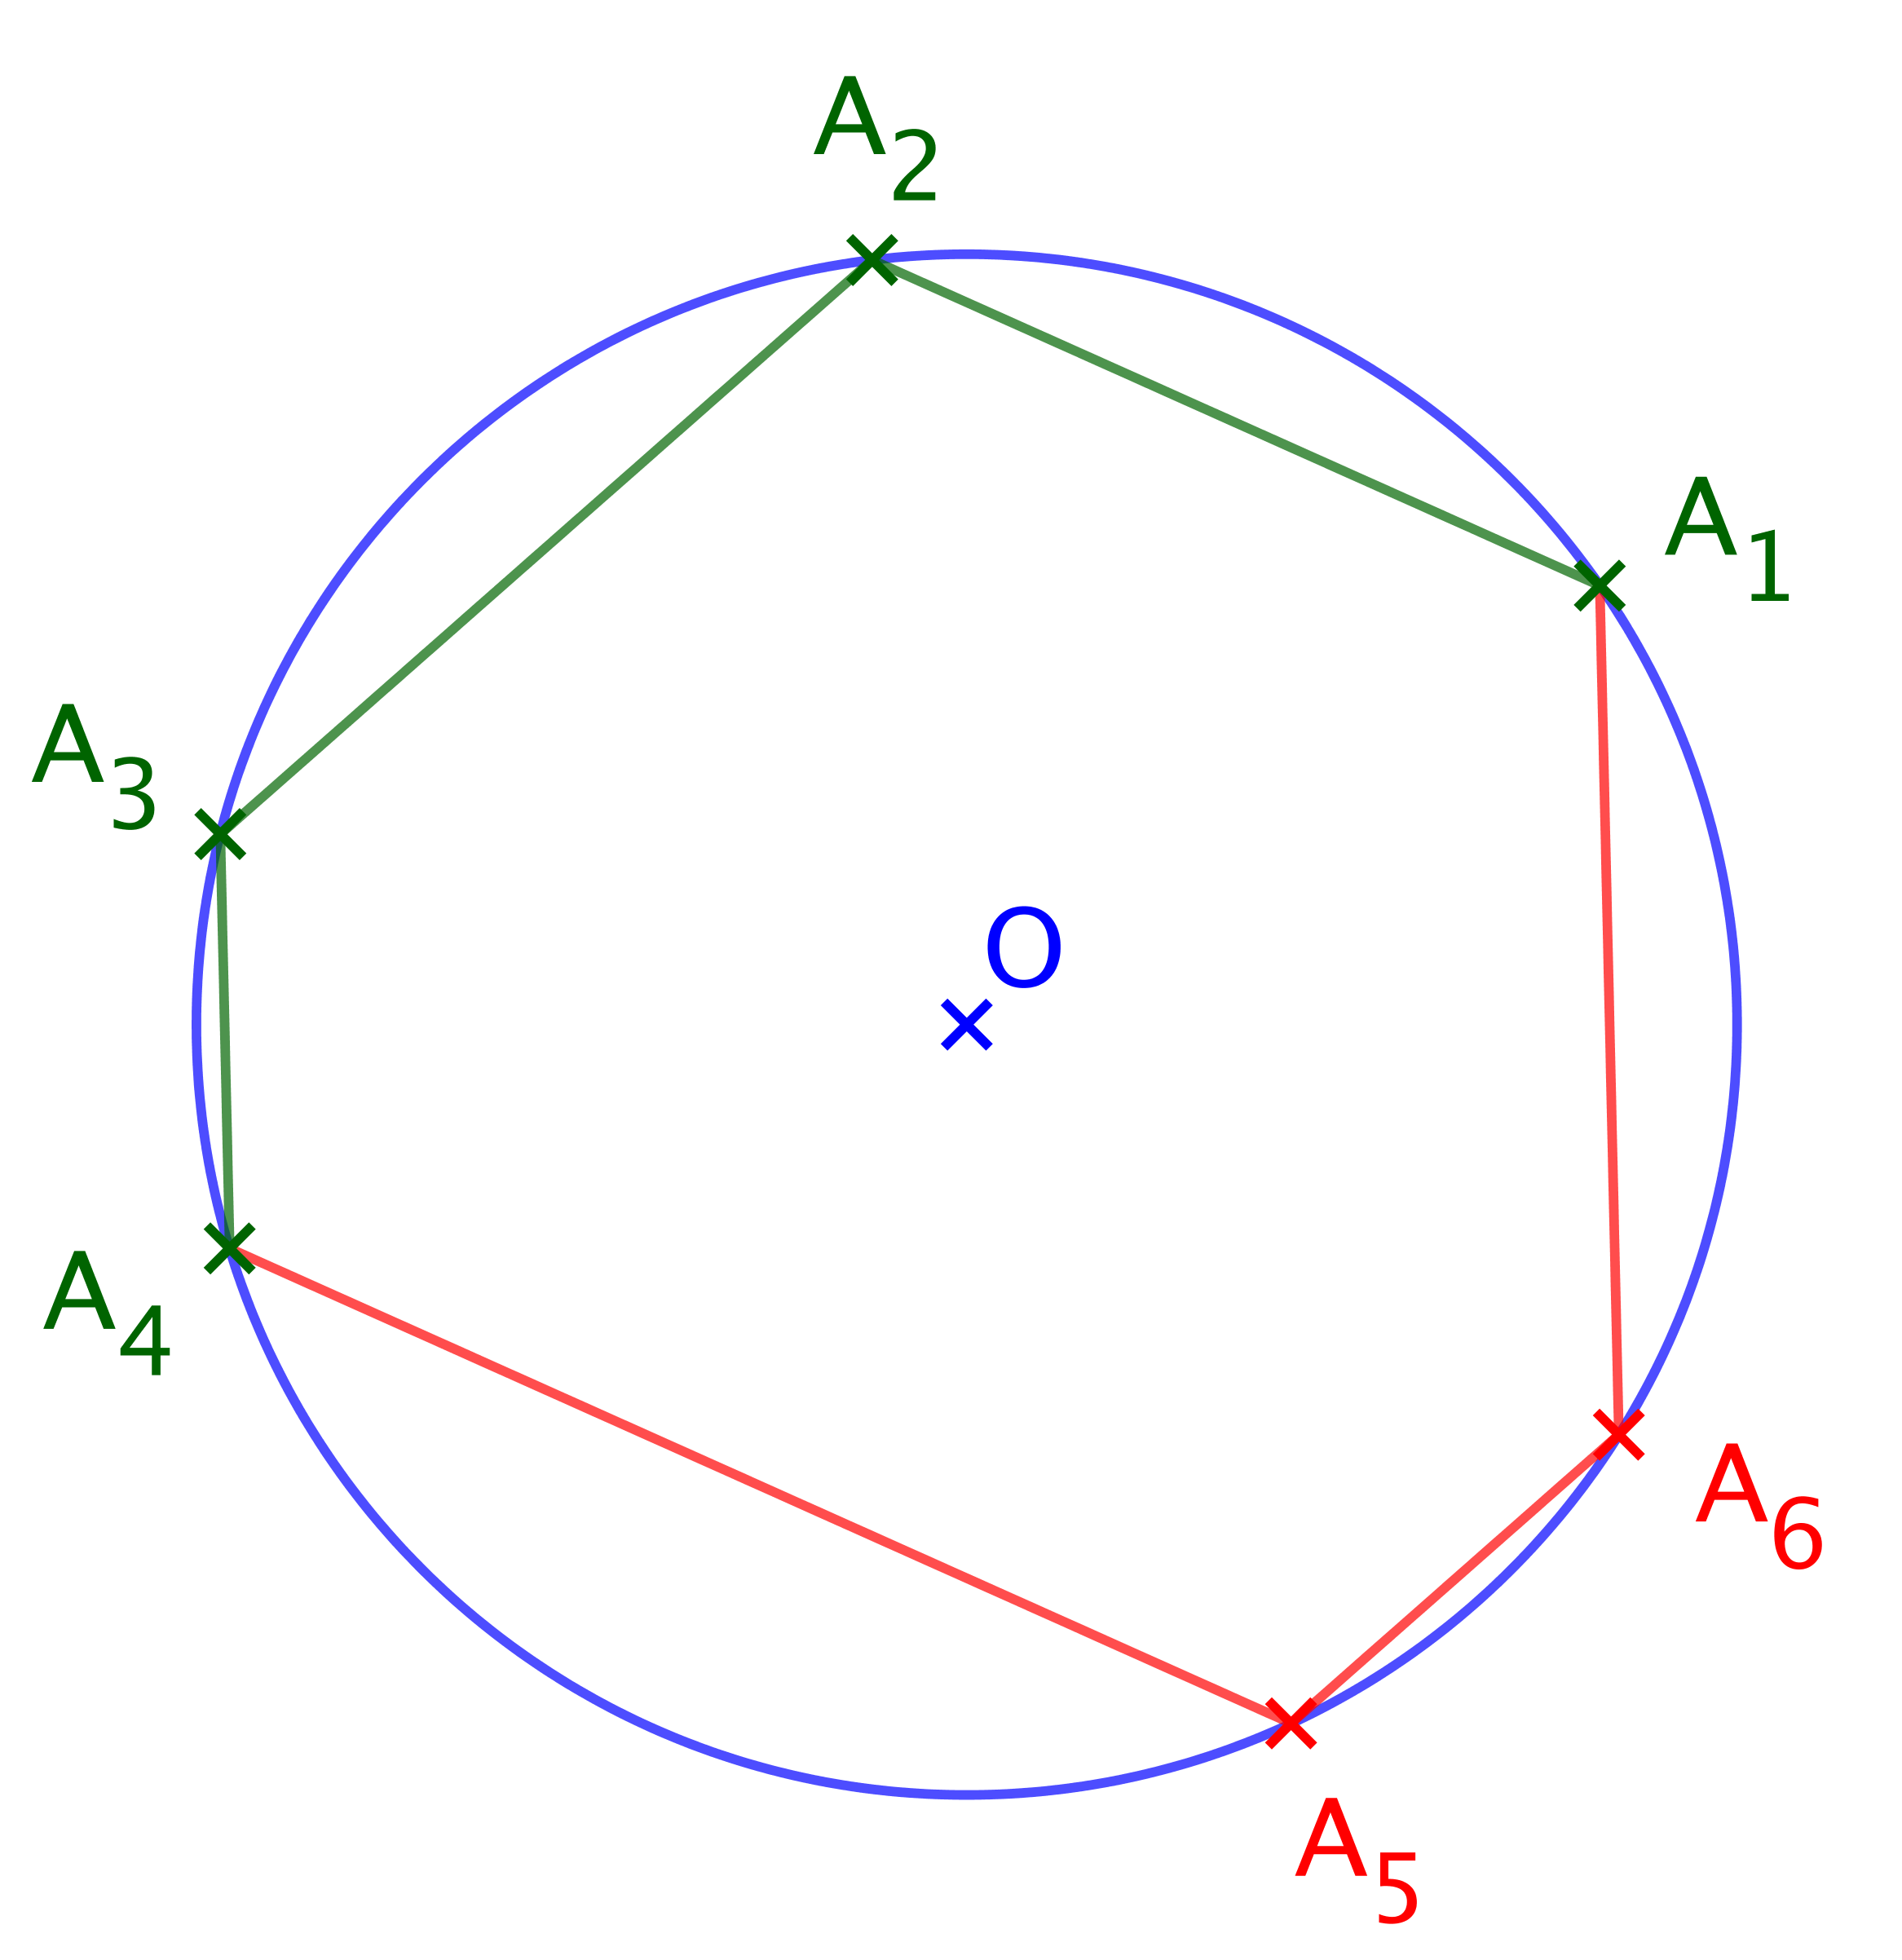
\includegraphics[scale = .6]{convex.png}}

	\columnbreak

	\fbox{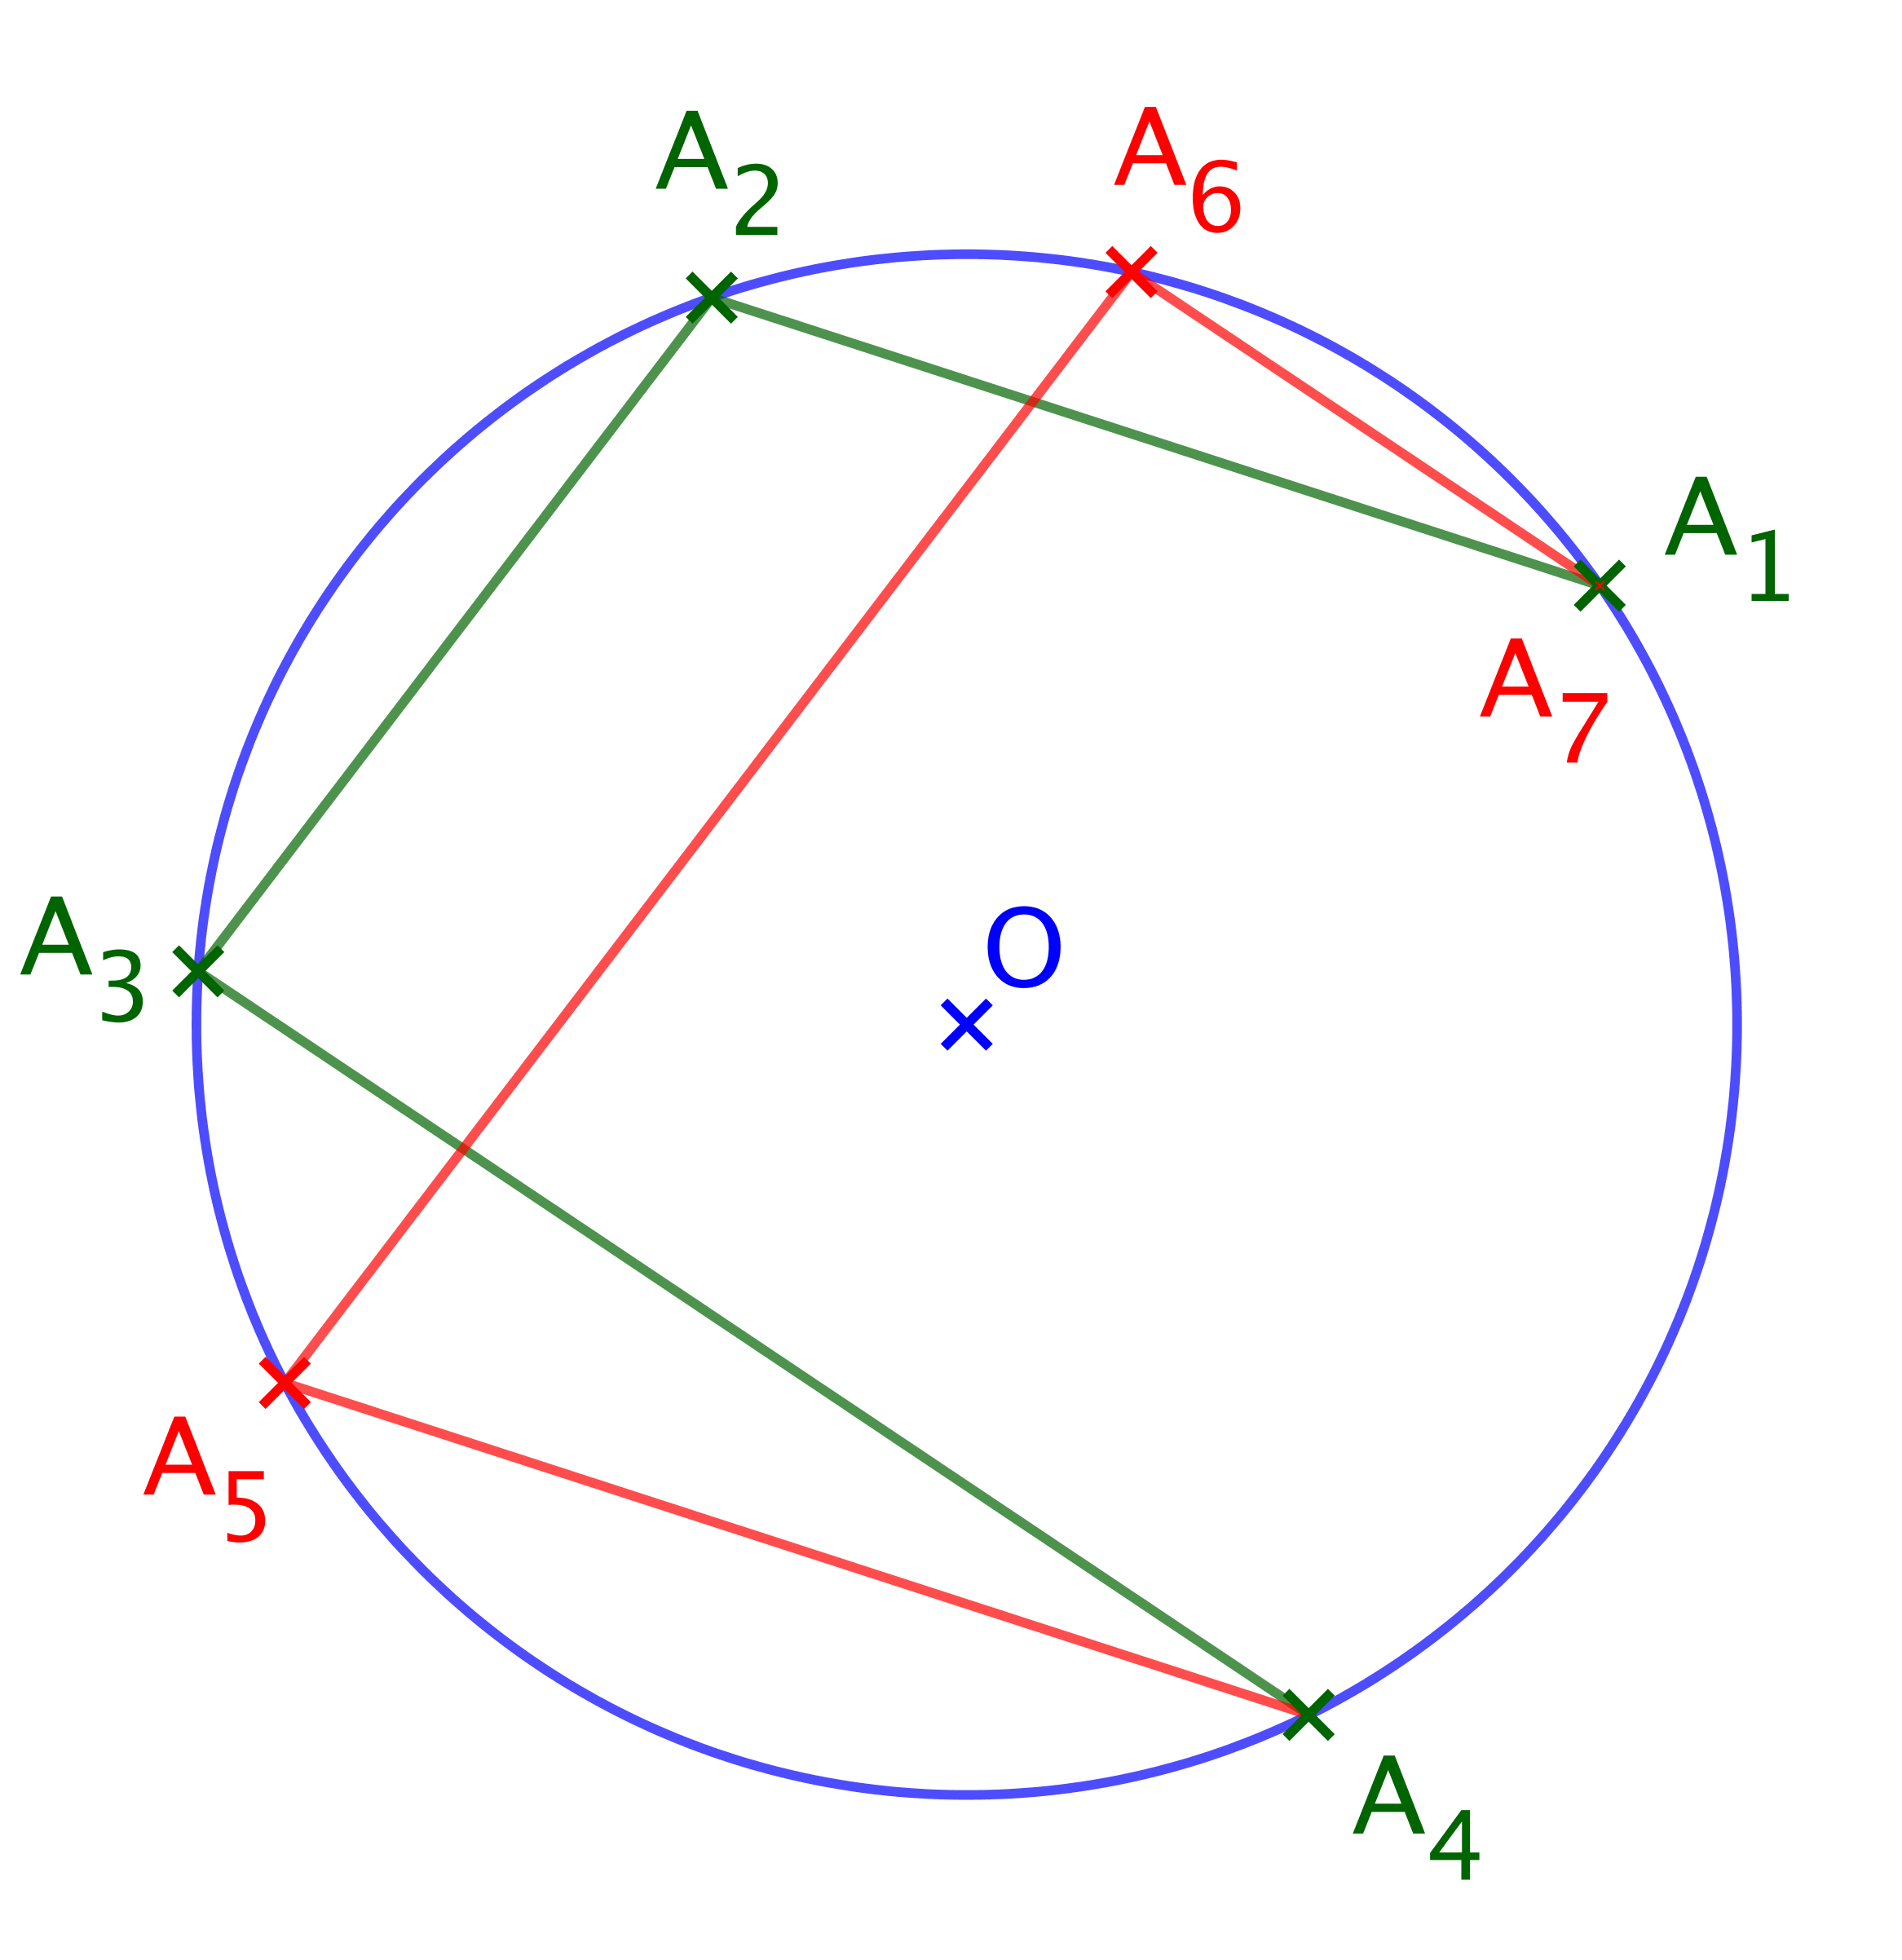
\includegraphics[scale = .6]{unconvex.png}}
\end{multicols}
